%=================================================================
\section{Motivation}

%-----------------------------------------------------------------
%\subsection{This is a subsection}
\begin{frame}
	\frametitle{Motivation}
	\begin{itemize} \myspacing
		\item Huge amount of clinical data produced over the years
		\item Different content types
		\begin{itemize}
			\item Unstructured and semi-structured texts
			\item Numeric and coded data
			\item Biosignals and images
		\end{itemize}
		\item Clinical text
		\begin{itemize}
			\item Short forms: abbreviations, acronyms
			\item Spelling and typing errors
			\item Short, incomplete sentences
		\end{itemize}
		\item Interesting scenarios
		\begin{itemize}
			%\item ``Similar patient'' retrieval
			\item Cross-patient search: cohort building for clinical trials
			\item ``Quick view'': displaying relevant clinical statements
		\end{itemize}
%		\item Two problems addressed 
%		\begin{itemize}
%			\item Unsupervised expansion of ad-hoc abbreviations in EHR narratives
%			\item Automated classification of pathology reports into ICD-O codes 
%		\end{itemize}
	\end{itemize}
\end{frame}

\begin{frame}
	\frametitle{Motivation}
                \begin{figure}
        			\centering
        			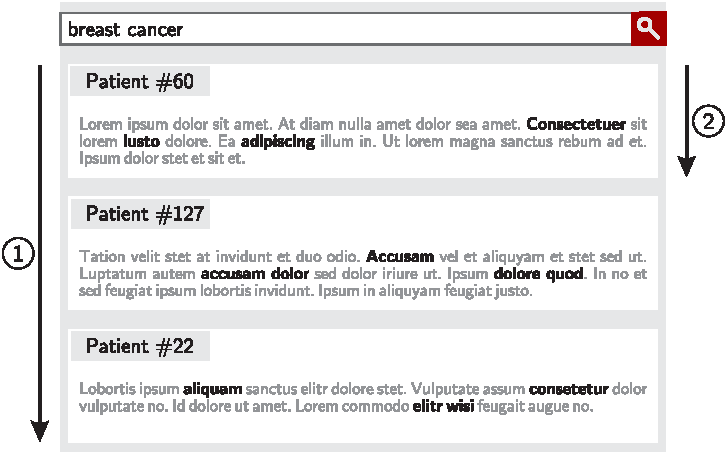
\includegraphics[width=10cm]{research_questions.pdf}
        			\caption{Interesting scenarios.}
        			\label{fig:research_questions}
  		\end{figure}
\end{frame}
